\chapter{Methodology}
\label{ch:method}

\section{Overview}
This chapter explains how we built the dataset, engineered features from the ZHVI time series and ACS data, and trained and evaluated our models. All work was done in Python using \texttt{pandas}, \texttt{scikit-learn}, and \texttt{matplotlib}. Our focus was on building a predictive setup that avoided target leakage and relied only on information available at the cutoff year.

\section{Data sources and filtering}
We used two main data sources:

\begin{itemize}
    \item \textbf{Zillow Home Value Index (ZHVI)}: Monthly home value estimates by ZIP code, accessed from Zillow’s data portal~\cite{zillow_data}.
    
    \item \textbf{American Community Survey (ACS)}: County-level demographic and economic data from the U.S. Census Bureau, accessed through their data portal~\cite{acs_data}.
\end{itemize}

We filtered the ZHVI data to only include ZIPs in Georgia, removed rows with missing city or metro names, and excluded ZIPs with more than 12 consecutive months of missing values. For ZIPs missing metro data, we filled it based on the most common metro for the city or county, unless the city was ambiguous.

The ACS data was pulled for all counties in Georgia. Since it is only available at the county level, each ZIP was assigned the values from its corresponding county for the matching year.

\section{Rolling dataset creation}
Each row in the final dataset represents a ZIP code and a year, using only data available up to the end of that year. We used a rolling window approach: for each ZIP-year pair, we created features from the historical ZHVI series leading up to December 31 of that year. If a ZIP didn’t have at least 24 months of usable data, we skipped it.

We interpolated missing values linearly and skipped any year where we couldn’t compute the YoY from the prior year. The final YoY value for the \textit{next} year was used as the target, meaning we are predicting one year ahead for each row.

\section{Feature engineering}
\subsection{ZHVI-based features}
From each ZIP’s historical ZHVI values, we extracted:
\begin{itemize}
    \item \texttt{FinalZHVI}: home value at the end of the year,
    \item \texttt{AvgMonthlyGrowth}: mean monthly growth in percent,
    \item \texttt{Volatility}: standard deviation of monthly growth,
    \item \texttt{CAGR}: compound annual growth rate since the start of the series,
    \item \texttt{NegativeGrowthYears}: count of past years with negative YoY growth,
    \item \texttt{YoY\_LastYear}: YoY growth from the previous year.
\end{itemize}

The target, \texttt{YoY\_target}, was the YoY growth from the current year to the next. For example, for a 2016 row, the target would be 2017’s growth.

\subsection{ACS-derived features}
Each ZIP inherited its county's ACS values. We engineered the following from raw ACS columns:
\begin{itemize}
    \item Percent renters, people below poverty, and households with no vehicle,
    \item Percent with a bachelor’s degree or higher,
    \item Unemployment rate,
    \item Household sizes (one-person and 4+),
    \item Age group breakdowns: percent ages 0–17, 18–34, and 65+.
\end{itemize}

For 2024, we forward-filled values using 2023’s ACS data since 2024 estimates were unavailable.

\section{Final dataset preparation}
Before modeling, we grouped rare county and metro names into an \texttt{Other} category to reduce sparsity, then one-hot encoded the remaining categorical columns.

To avoid leakage, we split the data by ZIP code rather than by row. That means if a ZIP appears in the training set, none of its years appear in the test set. This ensures the model isn’t learning from repeated geographic patterns across time.

We used data from the years 2011 through 2024, excluding 2020 due to unreliable ACS data during the COVID-19 pandemic. Although 2024 lacks observed target values, these rows were included in the final dataset for future forecasting. Only ZIP–year rows with valid targets were used for training and evaluation.

The final dataset had 3{,}009 rows and 139 columns, including both engineered and encoded features.

\section{Feature selection}
We used two methods to rank features:
\begin{itemize}
    \item \texttt{f\_regression}: measures linear correlation between each feature and the target,
    \item \texttt{mutual\_info\_regression}: detects both linear and non-linear dependencies.
\end{itemize}

We used the rankings to train models using the top $k$ features for $k$ from 1 to 50, comparing performance using 3-fold cross-validation.

\begin{figure}[!ht]
    \centering
    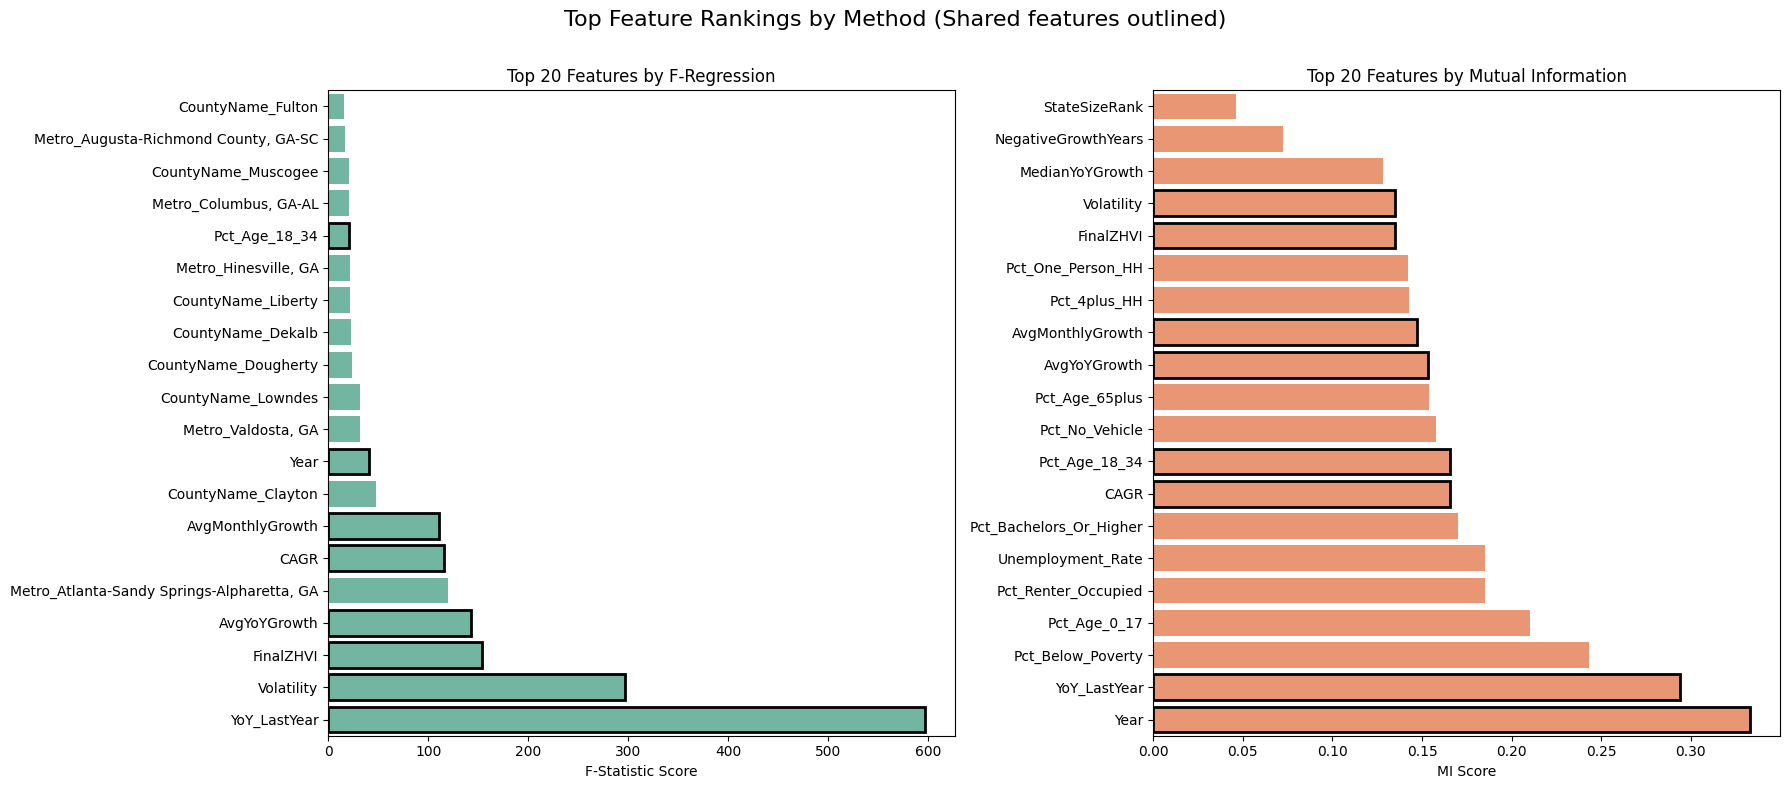
\includegraphics[width=\textwidth]{figures/topfeatures.png}
    \caption{Top 20 features by F-Regression and Mutual Information.}
    \label{fig:top_features}
\end{figure}
\FloatBarrier

Figure~\ref{fig:top_features} shows that features like \texttt{YoY\_LastYear}, \texttt{Volatility}, \texttt{FinalZHVI}, and \texttt{AvgMonthlyGrowth} were among the most informative. Mutual information also highlighted ACS features like poverty and education. These results suggest that both price history and local demographics contribute to future home value trends.

\section{Model training and evaluation}
We tested the following regression models:
\begin{itemize}
    \item Decision Tree,
    \item K-Nearest Neighbors,
    \item Random Forest.
\end{itemize}

Each model was tuned using \texttt{GridSearchCV}. We evaluated performance using:
\begin{itemize}
    \item $R^2$,
    \item RMSE,
    \item MAE,
    \item SMAPE.
\end{itemize}

Performance was reported on the held-out test ZIPs using both metrics and visual inspection of predictions.

\section{Ethical considerations}
The project uses only public datasets with no personal or identifiable information. All data is aggregated at the ZIP or county level. The models are for research and exploration only, and are not meant to support real-world financial decisions.

\section{Summary}
We filtered, cleaned, and reshaped housing data into a rolling ZIP–year format, added engineered time series and ACS features, and carefully split the data by geography to avoid leakage. After ranking features with two methods, we trained and evaluated three models using a consistent pipeline to understand what factors drive next-year home value growth.
